\chapter{Solución propuesta}
\label{chap:poc}

Como hemos comentado utilizaremos una librería de la segunda generación de criptografía homomórfica (Microsoft SEAL) y otra para la tercera (TFHE). Comenzaremos con un estudio del funcionamiento de las librerías, de cuales son sus límites computacionales y finalmente implementaremos una operación "no trivial" que requiera la utilización de ambas tecnologías.

La librería SEAL cuenta con pocas operaciones aritméticas implementadas, pero ofrece la posibilidad de trabajar con matrices y números decimales. La principal complicación con SEAL es determinar cómo se está desviando el cálculo para saber cuándo parar o qué correcciones hacer. Además, el número de operaciones que puede hacer son muy limitadas (cuando se hacen, por ejemplo productos, crece mucho el error). Además, el algoritmo que se implemente en SEAL no puede contener más que sumas, restas y multiplicaciones (no existe la división).

La librería TFHE ofrece una API de operaciones lógicas a nivel de bit. Aunque permitirá hacer cálculos más complejos sin añadir error al resultado, tendremos que implementar todas las operaciones a bajo nivel mediante puertas lógicas, siempre teniendo en cuenta que en ningún momento vamos a poder controlar el flujo de ejecución y nuestros algoritmos tienen que ser capaces de realizar los cálculos sin poder evaluar las variables (están cifradas).

Por lo tanto tenemos que encontrar un cálculo que sea realizable con pocas operaciones y números bajos para SEAL; y operaciones que sean implementables en un tiempo razonable con puertas lógicas para poder trabajar en TFHE.

Se han elegido tanto el sistema de ejemplo como las tecnologías específicas para cada uno de los actores en función de las capacidades y limitaciones de cada tecnología. Como resultado del proyecto se ha creado, además del análisis y el propio código del proyecto, una librería de operaciones matemáticas implementadas en TFHE (\cite{junquera_tfhe_2019}) con puertas lógicas, que es innovadora en tanto en cuanto no existe ningún código público que permita trabajar con TFHE a este nivel.

\section{Funcionamiento del sistema}

Para analizar las librerías implementaremos un sistema de posicionamiento anónimo en función de la temperatura y el mes del año. La base para determinar la posición serán dos curvas de regresión cuadrática de temperaturas de dos ciudades (generada con TFHE), que permitirá que un usuario suba a SEAL la fecha y la temperatura cifradas y averigüe su localización.

En este sistema habrá tres actores: el cliente, el servidor de posicionamiento (programado con SEAL) y un tercer servidor (programado con TFHE) que generará el modelo para calcular la posición. El cliente consultará su posición con el servidor de SEAL, que previamente habrá generado en el servidor de TFHE un modelo de posicionamiento basado en las temperaturas del último año en varias ubicaciones (ver \ref{fig:sistema_completo}).

Generaremos dicho modelo (la curva de regresión $f(x)$) con TFHE porque para ello necesitaremos realizar operaciones aritméticas que no nos ofrece SEAL. De esta forma, podremos realizar la evaluación de los datos introducidos por el usuario con SEAL (distancia entre el valor de temperatura $y$ especificado por el usuario, y $f(x)$ con $x$ el mes del año) utilizando sus operaciones más básicas, y aprovechando su sistema de vectores para evaluar todas las curvas al mismo tiempo.

\begin{figure}[h]
    \caption{Flujo de los datos cifrados\footnote{Diagrama generado con Piktochart \url{https://piktochart.com}}}
    \label{fig:sistema_completo}
    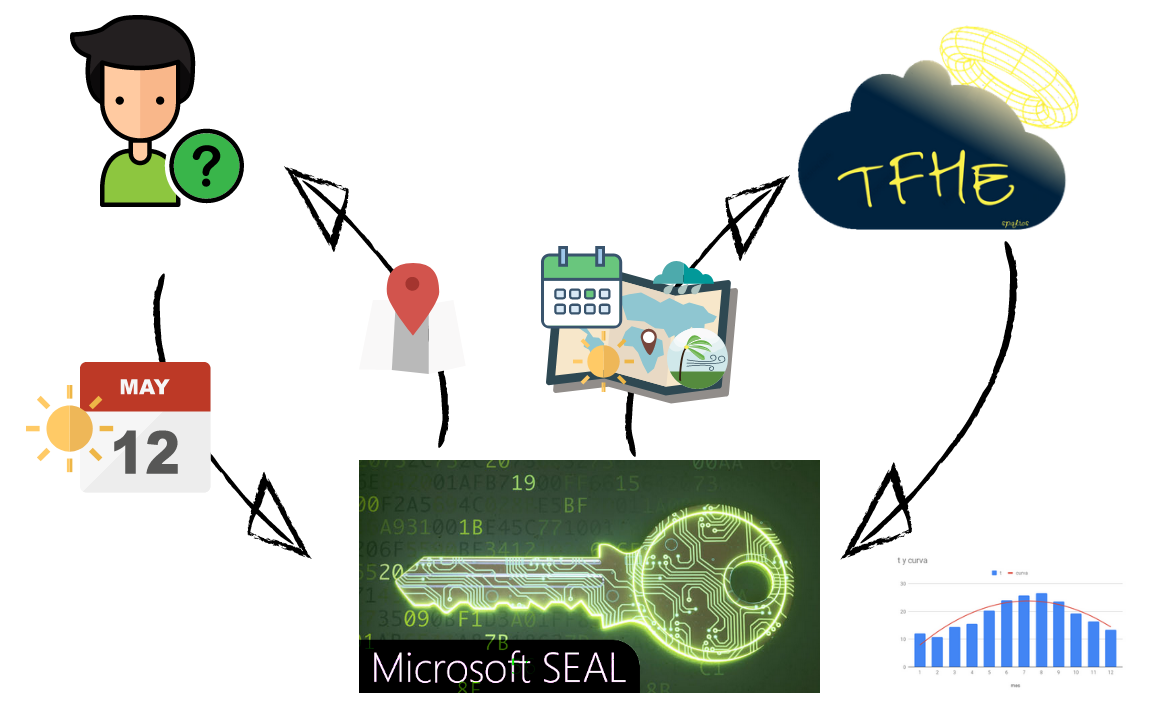
\includegraphics[width=\linewidth]{sistema_completo}
\end{figure}

\subsection{Generación del modelo}

Para generar el modelo el cliente (en este caso, el servidor de posicionamiento con SEAL) y el servidor (el servidor con TFHE) seguirían el siguiente procedimiento:

\begin{enumerate}
    \item El cliente genera un par de claves (pública y privada).

    \item Cifra $n$ pares de datos (en nuestro ejemplo el par sería $(mes, temperatura)$).

    \item Sube los datos cifrados y su clave pública. El número de datos que se puede subir está limitado por el crecimiento del tamaño (en bits) de dichos datos al exponenciarlos para calcular la curva de regresión. Trabajaremos con los datos de 12 meses porque, como comentaremos más adelante\ref{chap:resultados}, aunque el orden máximo al que llegaríamos con estos datos es de 46 bits tendremos otras limitaciones a la hora de procesar los datos.

    \item El servidor procesa los datos y devuelve cifrados los parámetros de la curva

    \item El cliente los descifra y los almacena asociados a una posición geográfica
\end{enumerate}

Finalmente, con los parámetros recibidos, el cliente obtendría una curva similar a \ref{fig:reg2_cg}.

\begin{figure}[h]
    \caption{Curva de Regresión Cuadrática con temperaturas de Cabo de Gata}
    \label{fig:reg2_cg}
    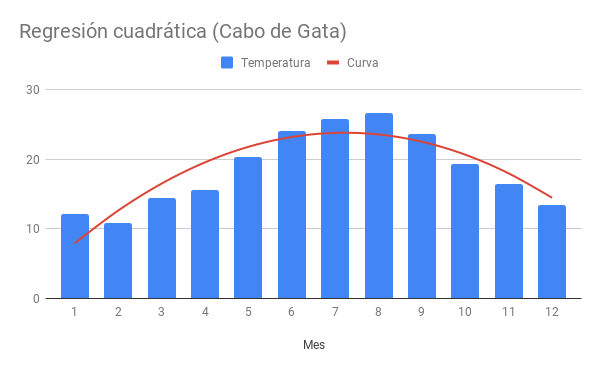
\includegraphics[width=\linewidth]{reg2_cg}
\end{figure}

\subsection{Obtención de la posición}

Teniendo el servidor de SEAL ya generados los modelos de la temperatura de cada ubicación (en este caso, sólo los 2 de Cabo de Gata y Finisterre) el cliente (ahora ya sí, el usuario final) consultará su ubicación:

\begin{enumerate}

  \item El cliente genera tres claves: pública, privada y clave de realinearización.

  \item El cliente cifra (con su clave pública) la temperatura y el mes del año para el que quiere hacer la consulta, generando los valores $y$ e $x$ respectivamente.

  \item Sube ambos valores al servidor, junto con la clave de realinearización (en nuestro ejemplo, no se necesitará subir la pública).

  \item El servidor calculará la diferencia (resta) entre el punto $y$ y $f(x)$ para cada curva

  \item El servidor devuelve una lista con los valores calculados y la ubicación a la que corresponde cada valor

  \item El cliente descifra los valores con su clave privada, obteniendo la distancia entre la temperatura introducida y el valor de la curva de cada una de las ubicaciones ese mes.

\end{enumerate}

En la figura \ref{fig:t_vs_r2} se puede ver un ejemplo del funcionamiento del sistema de posicionamiento. Los puntos introducidos corresponden a las temperaturas de varias ubicaciones, y el sistema de posicionamiento devolvería la distancia entre estos puntos y las dos curvas de regresión. De esta forma se puede obtener una estimación de la posición. En el ejemplo vemos que, la temperatura en Cabo de Gata está muy próxima a su curva en el mes de junio, y daría un resultado indeterminado en abril; que la temperatura de Madrid no casaría con ninguna de las dos curvas; o que la temperatura de Finisterre en noviembre efectivamente está mucho más cerca de la curva de Finisterre que de la de Cabo de Gata.

\begin{figure}[h]
    \caption{Temperatura vs Regresión}
    \label{fig:t_vs_r2}
    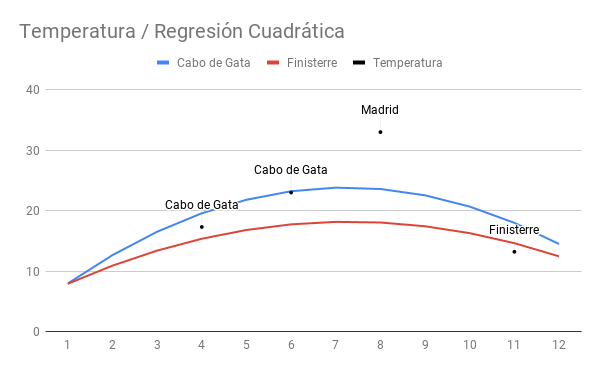
\includegraphics[width=\linewidth]{t_vs_r2}
\end{figure}

\section{Implementación con TFHE}

Para generar la curva de regresión que utilizará el servidor de SEAL para ubicar al usuario, dicho servidor cifrará los datos de temperatura del último año en dos ubicaciones distintas y se las enviará al servidor TFHE. Este procesa los datos cifrados y calcula la regresión cuadrática codificada en tres parámetros $a, b, c$ que devolverá cifrados al servidor de SEAL.

$ DIAGRAMA PARA SUBIR DATOS DE SEAL A TFHE$

\subsection{Curva de regresión}

Esta curva $ y = f(x) $ está definida por tres parámetros ($a$, $b$ y $c$) de forma que:

\[ y = ax^2 + bx + c \]

Resultante de resolver el siguiente sistema de ecuaciones:

\begin{gather*}
    \begin{cases}
        \sum_{i=0}^n y_i = a*\sum_{i=0}^n x_i^2 + b*\sum_{i=0}^n x_i + n*c \\
        \sum_{i=0}^n y_i = a*\sum_{i=0}^n x_i^3 + b*\sum_{i=0}^n x_i^2 + c*\sum_{i=0}^n x_i \\
        \sum_{i=0}^n y_i = a*\sum_{i=0}^n x_i^4 + b*\sum_{i=0}^n x_i^3 + c*\sum_{i=0}^n x_i^2
    \end{cases}
\end{gather*}

Realizando las siguientes sustituciones:

\begin{align*}
    i &= \sum_{i=0}^n x_i & j &= \sum_{i=0}^n x_i^2 & k &= \sum_{i=0}^n x_i^3 & l &= \sum_{i=0}^n x_i^4 \\
    u &= \sum_{i=0}^n y_i & v &= \sum_{i=0}^n x_i * y_i & w &= \sum_{i=0}^n x_i^2 * y_i
\end{align*}

Obtendríamos un sistema lineal de ecuaciones solucionable mediante eliminación Gauss-Jordan:

\begin{gather*}
    \begin{cases}
        u = a*j + b*i + n*c \\
        v = a*k + b*j + c*i \\
        w = a*l + b*k + c*j
    \end{cases}
\end{gather*}

Además de la propia implementación con TFHE (codificada en el apéndice \ref{appendix:reg2.cpp}), se ha desarrollado un código de ejemplo en python mucho más legible \ref{appendix:regresion_cuadratica.py}.

TFHE sólo ofrece operadores lógicos, así que tenemos que escribir la operaciones aritméticas necesarias: suma, resta, multiplicación y división. Además tendremos que dar la posibilidad de trabajar con números reales, por lo que tendremos que determinar la codificación más apropiada. Para todo ello se ha desarrollado la librería \texttt{tfhe-math}

\subsection{tfhe-math}

Código fuente en: \url{https://gitlab.com/junquera/tfhe-math}

El desarrollo de esta librería ha sido quizás la parte más costosa del trabajo, pero también la que más resultados arroja sobre la implementación de criptografía homomórfica en un entorno real. Como hemos comentado, hemos desarrollado las operaciones aritméticas necesarias para poder realizar la regresión cuadrática teniendo en cuenta que necesitábamos codificar los valores como número reales.

TFHE sólo trabaja con arrays de bits cifrados, y los datos no se pueden evaluar durante la ejecución del programa, así que hemos tenido que meter algunas funciones redundantes para cubrir todos los supuestos: Por ejemplo, en la multiplicación trabajamos asumiendo que los dos factores tienen signo positivo y corregimos el resultado utilizando la puerta lógica \texttt{MUX}. Por otro lado, como hay algunos casos en los que vamos a tener la certeza del signo de los operandos (porque lo hemos gestionado ya antes), y la lógica de tratamiento del signo es muy pesada, hemos creado algunas funciones para trabajar con números sin signo, cuyo nombre hemos precedido de \texttt{u\_} (de \textit{unsigned}).

A la hora de trabajar con los números con coma flotante, para proteger los decimales al codificar el número como entero, les asignamos un número determinado de bits. Por defecto, cuando trabajamos con números de 64 bits, les asignamos 10 (y así podemos guardar 3 decimales). Así por ejemplo, si queremos trabajar con el número $ 3.14 $, lo multiplicamos por $ 1024 $ ($ 2^{10} $, el equivalente a moverlo 10 bits hacia la izquierda) y trabajamos con $ 3215 $.

% TODO POner ejemplo de 3.14 * 1.4

Lo hacemos de esta forma (en lugar de, por ejemplo, multiplicar por 10) porque la operación de desplazamiento de bits es casi gratuita (en cuanto a tiempo de cómputo), mientras que la multiplicación y la división son muy costosas. Cuantos más bits introduzcamos, obtendremos mayor precisión, pero bajará la eficiencia.

Tenemos que tener precaución principalmente en dos aspectos:

\begin{enumerate}

  \item En el producto y en la división también se multiplican y dividen los desplazamientos. Por ejemplo si trabajamos con dos números ($a$ y $b$) a los que les hemos aplicado el desplazamiento de 10 bits ($ a' = a * 2^{10}, b' = b * 2^{10} $). Hay que restaurar la escala antes de la división:

  \begin{gather}
    \label{form:float_bits_product}
    a' / b' = ( a * 2^{10} ) / ( b * 2^{10} ) = (a / b) \\
    (a / b) \neq (a / b) * 2^{10}
  \end{gather}

  Para que al restaurar el número no haya errores quitando las posiciones de los decimales:

  \begin{gather}
    a' / b' \rightarrow (a' * 2^{10})/b' = (a / b) * 2^{10}
  \end{gather}

  Y hay que restaurar la escala tras la multiplicación:

  \begin{gather}
    a' * b' = ( a * 2^{10} ) * ( b * 2^{10} ) = a * b * 2^{20} \\
    a * b * 2^{20} \neq a * b * 2^{10}
  \end{gather}

  Para, además de evitar errores al restaurar el número, no se produzcan desbordamientos (si $a$ es de 4 bits, y $b$ es de 3, $ a * b $ ocupará 7 bits):

  \begin{gather}
    a' * b' \rightarrow (a' * b') / 2^{10} = a * b * 2^{10}
  \end{gather}

  \item La gestión del signo

  Para trabajar con el signo de los números se codifican en complemento a 2 (\cite{wikipedia_contributors._complemento_2019}). En la suma y la resta podemos operar libremente, pero a la hora de hacer la división y el producto (nuevamente) hemos tenido que implementar algoritmos que "no entienden de signo".  Siempre que necesitamos trabajar con algoritmos sin signo, y como no podemos cambiar el flujo de ejecución en función del mismo (porque no podemos verlo), realizamos el siguiente proceso con cada operando:

  \begin{enumerate}
    \item Negamos el operando: Para ello hemos creado la función \texttt{negativo} que devuelve el negativo del número si es positivo, y el positivo si es negativo.
    \item Guardarmos (usando la puerta \texttt{MUX}) el mayor de los dos para asegurarnos de trabajar con el número en positivo
    \item Guardamos en un bit (cifrado, un bit que no vemos pero que \texttt{MUX} será capaz de interpretar) si el número es positivo (guardarmos \texttt{0}) o negativo (guardamos \texttt{1})
    \item Tras operar comparamos con la puerta \texttt{XOR} los bits que indican si los operandos eran positivos o negativos. Nos devolverá \texttt{0} sólo si ambos eran positivos o negativos, indicando que no hay que hacer ninguna corrección. Llamaremos a este bit \texttt{corrector}.
    \item Aplicamos la función \texttt{negativo} sobre el resultado, y esta vez determinamos (usando \texttt{MUX}) qué devolver con el parámetro \texttt{corrector}: Si es \texttt{1} devolvemos el resultado negado, si es \texttt{0} el mismo que ha devuelvo el cálculo.
  \end{enumerate}

\end{enumerate}

\subsubsection{Operaciones}

A continuación veremos cómo trabajan nuestras principales funciones:

\begin{itemize}
  \item \texttt{gte}

  Compara los \verb|nb_bits| bits de \verb|a| y \verb|b| y marcar el bit \verb|result| con el valor de la expresión lógica \verb|a >= b|.

  \begin{lstlisting}[language=c++]
  void gte(LweSample* result, const LweSample* a,
          const LweSample* b, const int nb_bits,
          const TFheGateBootstrappingCloudKeySet* bk);
  \end{lstlisting}

  \item \verb|is_negative|

  Devuelve el valor del bit más significativo de \verb|a| (que es \verb|1| si es negativo y \verb|0| si no por la codificación en complemento a 2).

  \begin{lstlisting}[language=c++]
  void is_negative(LweSample* result, const LweSample* a,
                    const int nb_bits,
                    const TFheGateBootstrappingCloudKeySet* bk);
  \end{lstlisting}

  \item \texttt{negativo}

  Realiza el cambio de valor de \verb|a| en complemento a 2: Niega todos los bits y suma 1 al resultado.

  \begin{lstlisting}[language=c++]
  void negativo(LweSample* result, const LweSample* a,
                const int nb_bits,
                const TFheGateBootstrappingCloudKeySet* bk);
  \end{lstlisting}


  \item \texttt{minimum} / \texttt{maximum}

  Guarda en \verb|result| el valor mínimo o máximo entre \verb|a| y \verb|b|.

  \begin{lstlisting}[language=c++]
  void minimum(LweSample* result, const LweSample* a,
               const LweSample* b, const int nb_bits,
               const TFheGateBootstrappingCloudKeySet* bk);
  void maximum(LweSample* result, const LweSample* a,
               const LweSample* b, const int nb_bits,
               const TFheGateBootstrappingCloudKeySet* bk);
  \end{lstlisting}

  \item \texttt{shiftl} / \texttt{shiftr}

  Almacena en \verb|result| el valor de \verb|a| desplazado (hacia la izquierda o la derecha) el número de veces especificado en \verb|posiciones|. Es equivalente a multiplicar (mover a la izquierda) o dividir (mover a la derecha) entre dos. La operación sin signo (con \verb|u_|) es casi instantánea, y el coste de la implementación normal es casi exclusivamente el de la gestión del signo.

  \begin{lstlisting}[language=c++]
  void shiftl(LweSample* result, const LweSample* a,
              const int posiciones, const int nb_bits,
              const TFheGateBootstrappingCloudKeySet* bk);
  void shiftr(LweSample* result, const LweSample* a,
              const int posiciones, const int nb_bits,
              const TFheGateBootstrappingCloudKeySet* bk);
  \end{lstlisting}

  \item \texttt{add} / \texttt{sub}

  \verb|add| suma \verb|a| y \verb|b|. \verb|sub| aplica la función \verb|negativo| sobre \verb|b| y luego suma \verb|a| y \verb|-b|.

  \begin{lstlisting}[language=c++]
  void add(LweSample* result, const LweSample* a,
           const LweSample* b, const int nb_bits,
           const TFheGateBootstrappingCloudKeySet* bk);
  void sub(LweSample* result, const LweSample* a,
           const LweSample* b, const int nb_bits,
           const TFheGateBootstrappingCloudKeySet* bk);
  \end{lstlisting}

  \item \texttt{mult}

  Operación de multiplicación (ver figura \ref{fig:mult_float}). A diferencia de las anteriores, esta operación y \verb|div_float| tienen en cuenta los bits asignados a los decimales mediante el protocolo comentado anteriormente (ver \ref{form:float_bits_product}).

  \begin{lstlisting}[language=c++]
  void mult_float(LweSample* result,
                  const LweSample* a, const LweSample* b,
                  const int float_bits, const int nb_bits,
                  const TFheGateBootstrappingCloudKeySet* bk);
  \end{lstlisting}

  %
  % void mult(a, b){
  %
  %   // Multiplica opA * opB
  %   for(int i = 0; i < (nb_bits/2); i++) {
  %
  %     for(int j = 0; j < (nb_bits/2) + 1; j++)
  %       bootsAND(&aux[j+i] , &a[i], &b[j], bk);
  %
  %     add(result, aux, result, nb_bits, bk);
  %
  %   }
  % }
  %
  \begin{figure}[h]
    \caption{Algoritmo de multiplicación}
    \label{fig:mult_float}
    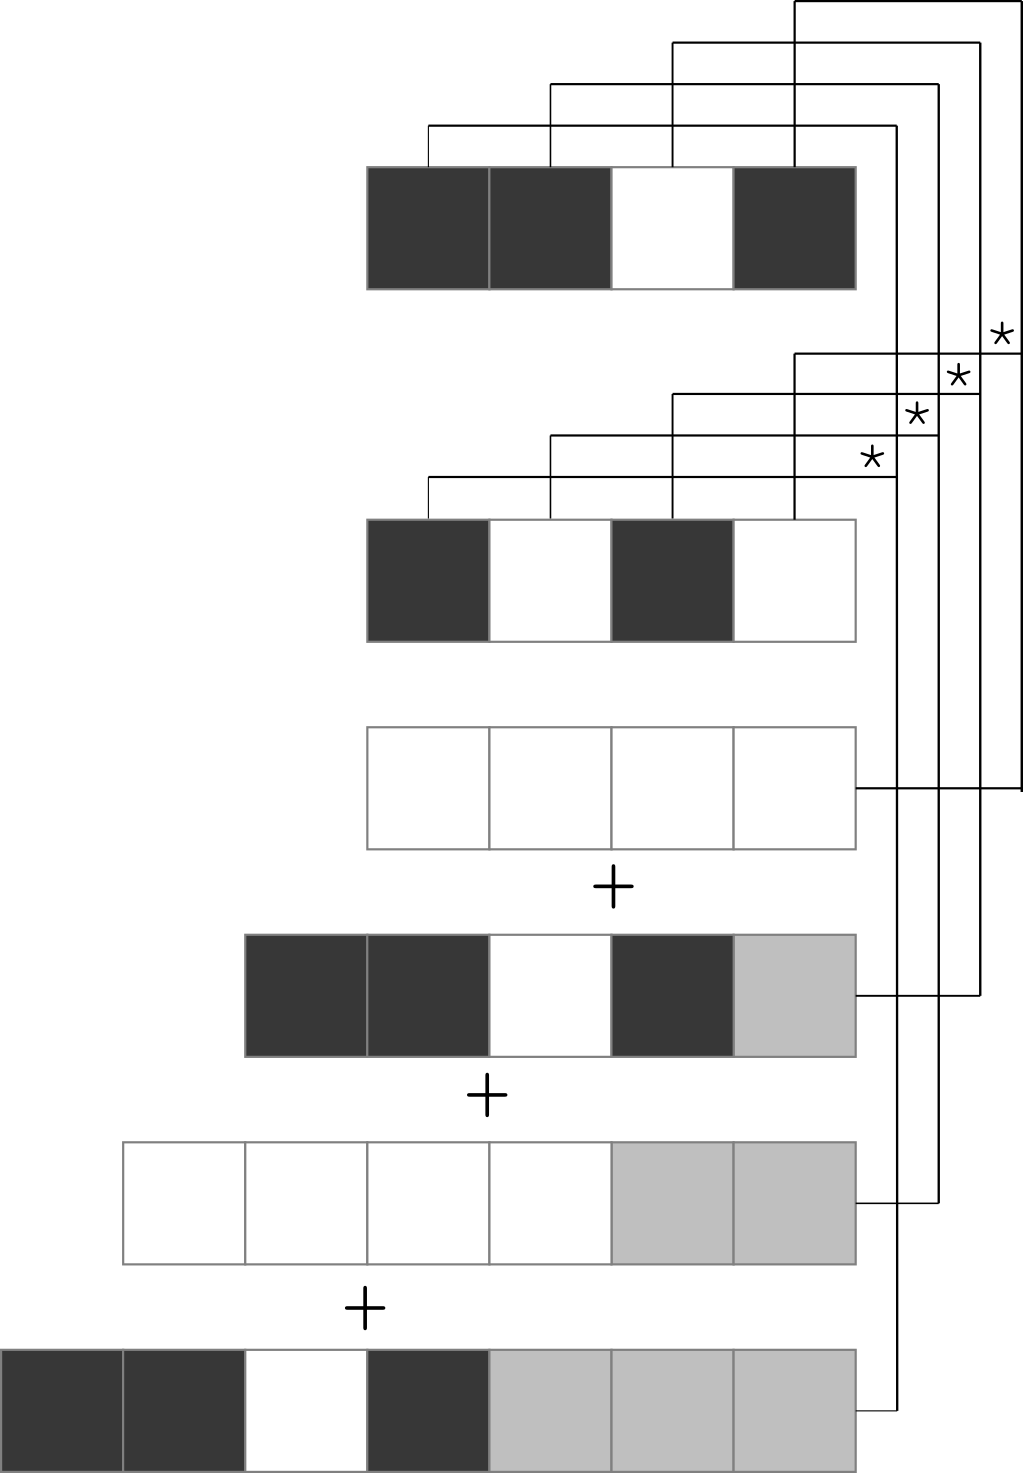
\includegraphics[width=\textwidth]{mult_float}
  \end{figure}

  \item \texttt{div}

  Operación de división (ver figura \ref{fig:div_float}). Es la operación más costosa porque requiere duplicar el tamaño (en bits) de los elementos, pero es esencial para realizar nuestro cálculo, y es el principal elemento que marca la diferencia con respecto al resto de implementaciones.

  \begin{lstlisting}[language=c++]
  void div_float(LweSample* result,
                  const LweSample* a, const LweSample* b,
                  const int float_bits, const int nb_bits,
                  const TFheGateBootstrappingCloudKeySet* bk);
  \end{lstlisting}

  %
  % void div(dividendo, b){
  %
  %   u_shiftl(divisor, b, nb_bits - 1, 2*nb_bits, bk);
  %
  %
  %
  %   for(int i = 0; i < nb_bits; i++) {
  %     // gt = dividendo >= divisor
  %     gte(gt, dividendo, divisor, 2*nb_bits, bk);
  %
  %     bootsCOPY(&cociente[nb_bits-i-1], &gt[0], bk);
  %
  %     // resto = gt? sub(dividendo, divisor) : resto
  %     sub(div_aux, dividendo, divisor, 2*nb_bits, bk);
  %     // divisor = shiftr(divisor, 1)
  %     u_shiftr(div_aux2, divisor, 1, 2*nb_bits, bk);
  %     for(int j = 0; j < 2*nb_bits; j++){
  %       bootsMUX(&resto[j], &gt[0], &div_aux[j], &dividendo[j], bk);
  %       // dividendo = gt ? resto : dividendo
  %       bootsMUX(&dividendo[j], &gt[0], &resto[j], &dividendo[j], bk);
  %       bootsCOPY(&divisor[j], &div_aux2[j], bk);
  %     }
  %   }
  % }
  %
  \begin{figure}[h]
    \caption{Algoritmo de división}
    \label{fig:div_float}
    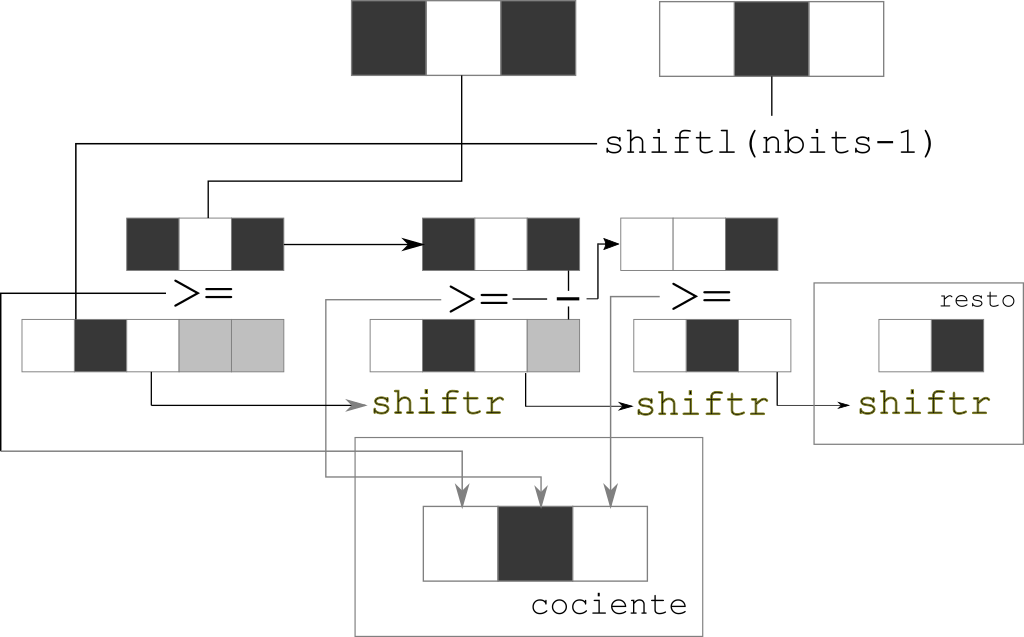
\includegraphics[width=\textwidth]{div_float}
  \end{figure}


\end{itemize}

\section{Implementación con SEAL}

\subsection{Cálculo de la posición}

El sistema CKKS ofrece la posibilidad de trabajar con varios datos a la vez codificándolos como vectores. Hemos aprovechado esta característica para poder resolver la distancia entre el punto introducido por el usuario y las distintas curvas en una sola llamada, aplicando las operaciones necesarias en todas las curvas al mismo tiempo.

Procedemos de la siguiente manera:

\begin{enumerate}
    \item Generamos un vector $A$ con los valores $a$ de todas las curvas, otro $B$ con los valores $b$ y otro $C$ con los valores $c$ de las curvas.
    \item Codificamos todos estos vectores con \verb|CKKSEncoder|

    \item Determinamos el punto $y$ correspondiente al valor $x$ introducido por el usuario.
    Como sólo podemos hacer una operación en cada paso, tenemos que descomponer la sustitución en varias operaciones. En cada producto, al estar utilizando el esquema CKKS, tendremos que reescalar (y realinearizar, cuando los cálculos pendientes así lo requieran) nuestro resultado. La operación de reescalado trunca el número (le quita bits, ver \ref{tag:ckks}) y modifica los parámetros de cifrado reduciendo el número de operaciones restantes que podemos realizar con él. Por lo tanto, hay que intentar realizar el menor número de productos posible. Por ejemplo, si hubiese que hacer la operación $x_4=x^4$, sería preferible hacer $x_2 = x^2, x_4 = x_2^2$ (con sólo dos productos) que $x_4 = x * x * x * x$ (con cuatro).

    Además, al realizar el reescalado estamos obteniendo un número con una escala menor que el número que hemos cifrado inicialmente, por lo que cuando queramos sumar dos variables tenemos que asegurarnos de ajustarlas entre sí o saltará una excepción. Estas operaciones realmente se corresponden con eliminar valores de una cadena que gestiona \verb|SEALContext| en la que se especifican los parámetros de cifrado de cada fase.

    Tras realizar este estudio, procedemos a calcular:
    \begin{enumerate}
        \item $p_1 = x^2$
        \item Realinearización y reescalado de $p_1$. Aquí realinearizamos porque este elemento es el que más productos va a tener ($ A * x^2$ conlleva tres productos, mientras que $B * x$ sólo uno).
        \item $p_2 = p_1 * A$
        \item Reescalado de $p_2$
        \item $p_3 = B*x$
        \item Reescalado de $p_3$
        \item $p = p_2 + p_3$
        \item Doble reescalado de $C$ para poder sumarlo con $p$
        \item $y = p + C$
    \end{enumerate}

    \begin{gather}
      \label{form:distancias_seal}
        \begin{pmatrix}
            d_1 \\
            d_2 \\
            \vdots{} \\
            d_n
        \end{pmatrix}
        =
        \begin{pmatrix}
            y \\
            y \\
            \vdots{} \\
            y
        \end{pmatrix}
        - (x^2 *
        \begin{pmatrix}
            a_1 \\
            a_2 \\
            \vdots{} \\
            a_n
        \end{pmatrix}
        + x *
        \begin{pmatrix}
            b_1 \\
            b_2 \\
            \vdots{} \\
            b_n
        \end{pmatrix}
        +
        \begin{pmatrix}
            c_1 \\
            c_2 \\
            \vdots{} \\
            c_n
        \end{pmatrix}
        )
    \end{gather}

    \item Finalmente, como nuestro $y$ es el resultado de dos reescalados, tendremos que reescalar dos veces el $y$ introducido por el usuario (al que llamaremos $y_0$) para poder operar. Tras hacerlo, devolvemos el resultado \verb|encrypted_result| igual a $y - y_0$.

\end{enumerate}

Cuando el usuario descifre \verb|encrypted_result|, obtendrá un vector con las distancias entre el punto que ha introducido y todas las curvas, similar al de la figura \ref{form:distancias_seal}.

\section{Implementaciones Cliente/Servidor}

Finalmente, para cada una de las tecnologías se han desarrollado dos programas que hacen las funciones de cliente y servidor. De esta forma separamos la lógica de cifrado y descifrado (perteneciente a los clientes) y la lógica de procesado de los datos cifrados (propia de los servidores).

Para ambas, se ha programado una clase cliente, y una clase servidor, como hemos comentado cada una con las funciones que le son propias por su rol en la arquitectura, y para el desarrollo del trabajo hemos creado cuatro ejecutables que, apoyándose en las clases cliente/servidor implementarán la lógica para generar la curva de regresión y evaluar en el resultado los valores. De ahora en adelante cuando hablemos de cliente y servidor nos referiremos a estos ejecutables.

\begin{itemize}

    \item TFHE
    
    Código fuente en: \url{https://gitlab.com/junquera/tfhe-cs}
    
    El cliente TFHE ofrece la posibilidad de:
    
    \begin{enumerate}
        \item Generar datos cifrados de la temperatura en Cabo de Gata guardando los $n$ valores de las $x$ con el formato \verb|ciudad_AXn.data| y los de las $y$ como  \verb|ciudad_AYn.data|).
        \item Generar datos cifrados de la temperatura en Finisterre siguiendo el mismo formato que anteriormente, pero con el prefijo \verb|ciudad_B|.
        \item Analizar los resultados generados por el servidor (indicándole la ruta en la que están, busca los archivos \verb|{a,b,c}.data|
        \item Descifrar un archivo cifrado con TFHE
    \end{enumerate}{}
    
    Cuando genera los datos cifrados, además exporta al sistema de archivos las claves para poder descifrar estos archivos cuando sea necesario, y poder subir la pública al servidor para procesar los datos.
    
    El módulo que hace las veces de servidor con TFHE generará los parámetros $a$, $b$ y $c$ de los que llevamos hablando toda la sección en base a los archivos \verb|ciudad_...| que haya en la carpeta que se le indique. Como el proceso es muy lento, almacenará los resultados de las operaciones intermedias para recurrir a ellos si se corta la ejecución (ver \ref{fig:resultados_tfhe}), hasta generar los archivos $a.data$, $b.data$ y $c.data$.

\begin{lstlisting}[caption=Archivos generados por el servidor, label=fig:resultados_tfhe]
junquera@opa:~/UEM/TFM/results/tfhe/ciudad_A/resultados$ ls -la
total 4240
drwxrwxr-x 2 junquera junquera   4096 ago 27 22:29 .
drwxrwxr-x 3 junquera junquera   4096 ago 16 10:06 ..
-rw-rw-r-- 1 junquera junquera 129024 ago 27 20:33 a.data
-rw-rw-r-- 1 junquera junquera 129024 ago 27 08:22 b.data
-rw-rw-r-- 1 junquera junquera 129024 ago 25 23:22 c.data
-rw-r--r-- 1 junquera junquera 129024 ago 16 10:06 i2.data
-rw-rw-r-- 1 junquera junquera 129024 ago 24 07:08 i2l2.data
...
-rw-rw-r-- 1 junquera junquera 129024 ago 23 20:06 ul.data
-rw-rw-r-- 1 junquera junquera 129024 ago 16 10:06 v.data
-rw-rw-r-- 1 junquera junquera 129024 ago 23 20:06 vl.data
-rw-rw-r-- 1 junquera junquera 129024 ago 16 10:06 w.data
-rw-rw-r-- 1 junquera junquera 129024 ago 23 20:06 wj.data
\end{lstlisting}

    Para hacer una prueba lo más realista posible de todo el sistema, he cifrado los datos que he obtenido de AEMET (ver \ref{appendix:datos_aemet}) de las temperaturas en las dos ciudades con el cliente de TFHE, y los he subido a la nube (DigitalOcean, \url{https://www.digitalocean.com/}) para procesarlos con el código del servidor TFHE.
    
    Tras finalizar el cálculo, los he descargado y descifrado con el cliente TFHE, y he insertado manualmente los resultados en el código del servidor SEAL. 

    \item SEAL
    
    Código fuente en: \url{https://gitlab.com/junquera/seal-cs}
    
    El servidor (\verb|server.main|) lee de la carpeta en la que se está ejecutando los archivos cifrados \verb|x.data| y \verb|y.data| generados por el cliente, y los elementos criptográficos necesarios (clave pública, clave de realinearización y parámetros de cifrado). Tras procesar estos datos con los valores de las curvas que ha calculado previamente en TFHE, genera el archivo \verb|result.data| y un archivo de texto con los nombres de las curvas (para que el cliente pueda interpretar los resultados).
    
    El \verb|main| del cliente (codificado en el archivo \verb|client-main.cpp|) tiene dos funcionalidades:
    \begin{enumerate}
        \item En la primera pide que se introduzcan dos valores (temperatura y fecha), los cifra y genera dos archivos: \verb|x.data| y \verb|y.data|.
        
        \item La otra funcionalidad, que se ejecuta tras la ejecución del código del servidor lee el archivo  \verb|result.data| de la carpeta en la que se ejecuta, lo descifra e imprime por pantalla el resultado combinado del vector descifrado con el archivo \verb|curve_names.data|. En \ref{fig:ejecuta_seal_cs} se puede ver la ejecución del sistema completo.
    
      \begin{figure}[h]
        \caption{Ejecución completa del sistema de SEAL}
        \label{fig:ejecuta_seal_cs}
        \centering
        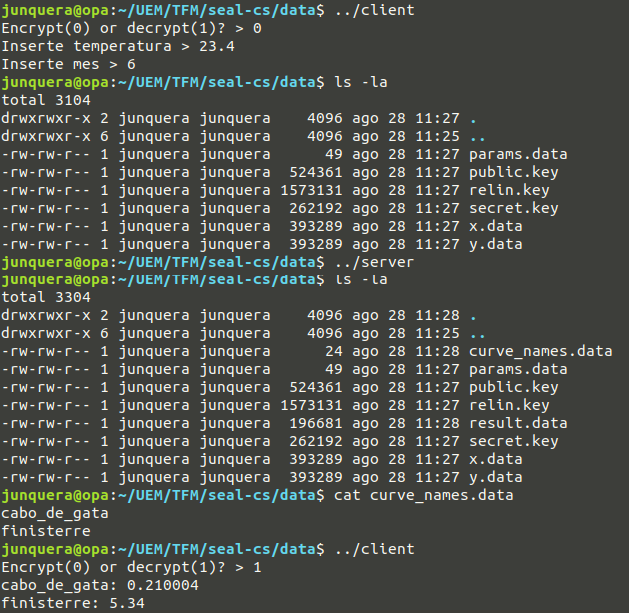
\includegraphics[width=0.75\textwidth]{ejecuta_seal_cs}
      \end{figure}
    \end{enumerate}{}
\end{itemize}

\section{Evaluación de límites y rendimientos}

Por último se han desarrollado varios archivos de prueba para evaluar los límites y el rendimiento de las librerías. Estas pruebas son la culminación de este estudio, y buscan aportar un enfoque cuantitativo a su funcionamiento, más allá de los cálculos que se puedan hacer con el conocimiento de las tecnologías o la visión empírica desde el punto de vista del desarrollador. Se ha evaluado:

\begin{itemize}
    \item TFHE
    Para evaluar la eficiencia de SEAL ejecutamos todas las funciones aritméticas que hemos escrito en \verb|tfhe-math| con distintos tamaños de texto cifrado (desde 4 hasta 64 bits) calculando el tiempo que tardan en realizarse. En el capítulo de resultados (\ref{chap:resultados}) veremos la comparativa entre los resultados obtenidos y el tiempo estimado en base a la teoría.
    \item SEAL
    Con SEAL hemos desarrollado dos tipos de pruebas:
    \begin{itemize}
        \item Al igual que con TFHE, hemos evaluado el tiempo que tarda en realizar las operaciones aritméticas (en este caso, sólo suma y multiplicación) con distintos tamaños de texto cifrado.
        \item También hemos evaluado cuáles son los límites de cómputo con distintos tamaños de texto cifrado, con y sin aplicar realinearizaciones.
    \end{itemize}
\end{itemize}

Ya sólo queda analizar los resultados de todos nuestros experimentos.